\documentclass[aspectratio=169]{beamer}

% Theme and color
\usetheme{Madrid}
\usecolortheme{default}

% Packages
\usepackage[utf8]{inputenc}
\usepackage[T1]{fontenc}
\usepackage{graphicx}
\usepackage{booktabs}
\usepackage{amsmath}
\usepackage{multirow}
\usepackage{hyperref}

% Custom colors
\definecolor{UnBBlue}{RGB}{0,61,165}
\setbeamercolor{structure}{fg=UnBBlue}
\setbeamercolor{title}{fg=white,bg=UnBBlue}
\setbeamercolor{frametitle}{fg=white,bg=UnBBlue}

% Title page information
\title[Layout-Aware ZSL for VDM]{Layout-Aware Zero-Shot Learning for Visual Document Matching}
\subtitle{Qualificação de Mestrado}
\author{Lucas de Almeida Bandeira Macedo}
\institute[UnB]{
    Universidade de Brasília\\
    Departamento de Ciência da Computação\\
    \vspace{0.3cm}
    Orientador: Prof. Dr. Pedro Garcia Freitas\\
    Coorientador: Prof. Dr. Bruno Luiggi Macchiavello Espinoza
}
\date{Outubro de 2025}

\begin{document}

% Title slide
\begin{frame}
\titlepage
\end{frame}

% Outline
\begin{frame}{Agenda}
\tableofcontents
\end{frame}

% Include sections
% ============================================
% SECTION 1: Introduction
% ============================================
\section{Introdução}

\begin{frame}{Contexto - Documentos e Compliance}
\begin{itemize}
    \item Documentos físicos
    \item Imagens de documentos
    \item Exemplos:
    % \begin{itemize}
    %     \item Carteira de identidade
    %     \item Carteira de habilitação
    %     \item Recibos
    %     \item Contratos
    % \end{itemize}
    \begin{center}
    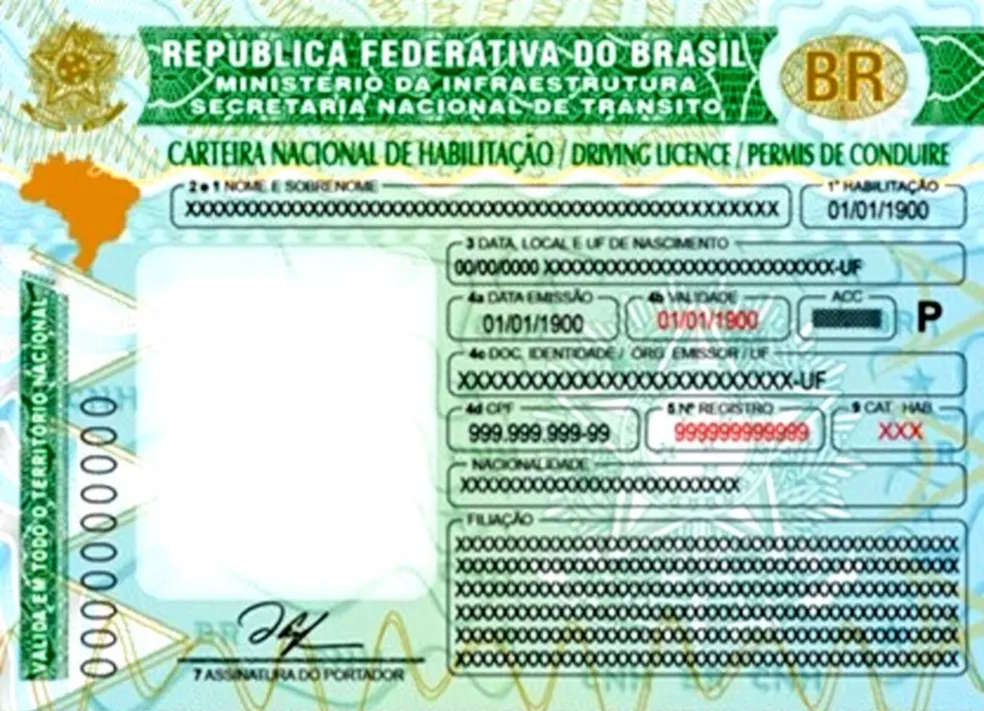
\includegraphics[width=0.27\textwidth]{images-apresentacao/CNH_EXEMPLO.jpg}
    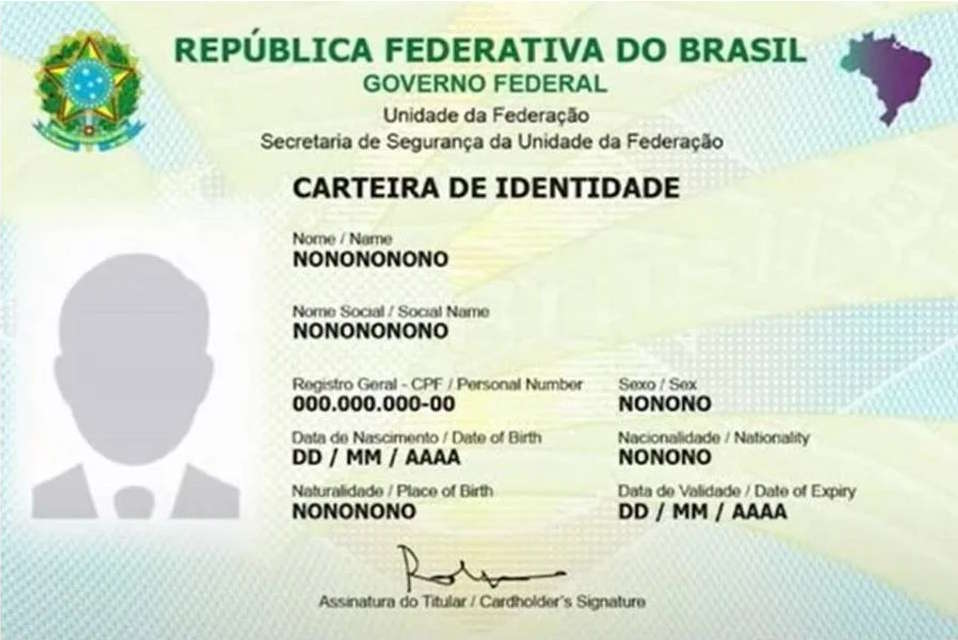
\includegraphics[width=0.29\textwidth]{images-apresentacao/CIN_EXEMPLO.jpg}
    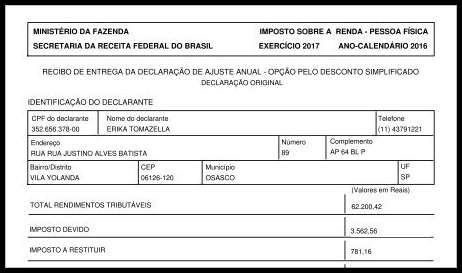
\includegraphics[width=0.33\textwidth]{images-apresentacao/IRPF_EXEMPLO.jpg}
\end{center}
\end{itemize}
\end{frame}


\begin{frame}{Contexto - Processamento de Documentos}
\begin{center}
% Sobreposição de imagens usando tikz
\begin{tikzpicture}
    % Imagem de fundo (diagrama)
    \node[anchor=center] at (0,0) {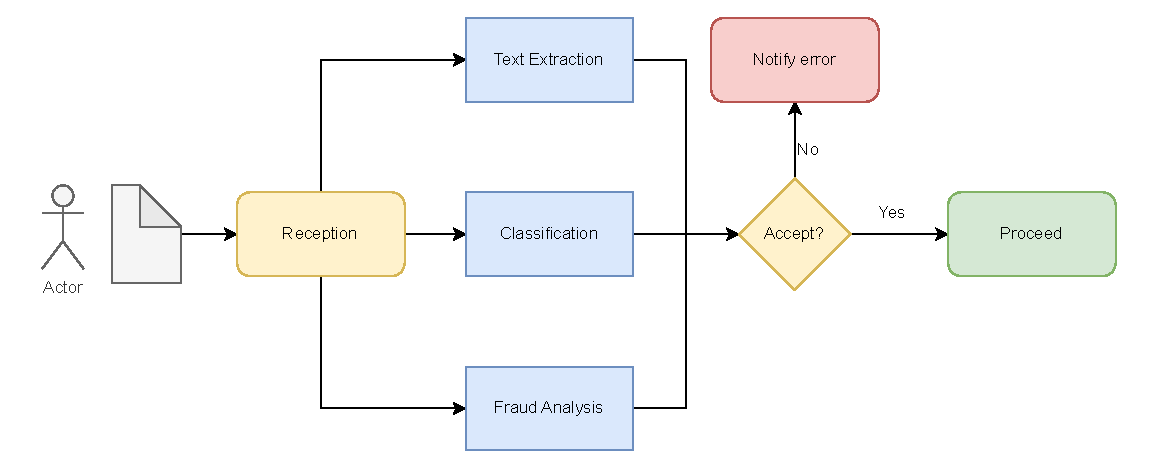
\includegraphics[width=1\textwidth]{images/diagrama-compliance.drawio.pdf}};
    
    % Imagem sobreposta (documento) - ajuste a posição (x,y) conforme necessário
    \node[anchor=center] at (-6,2.5) {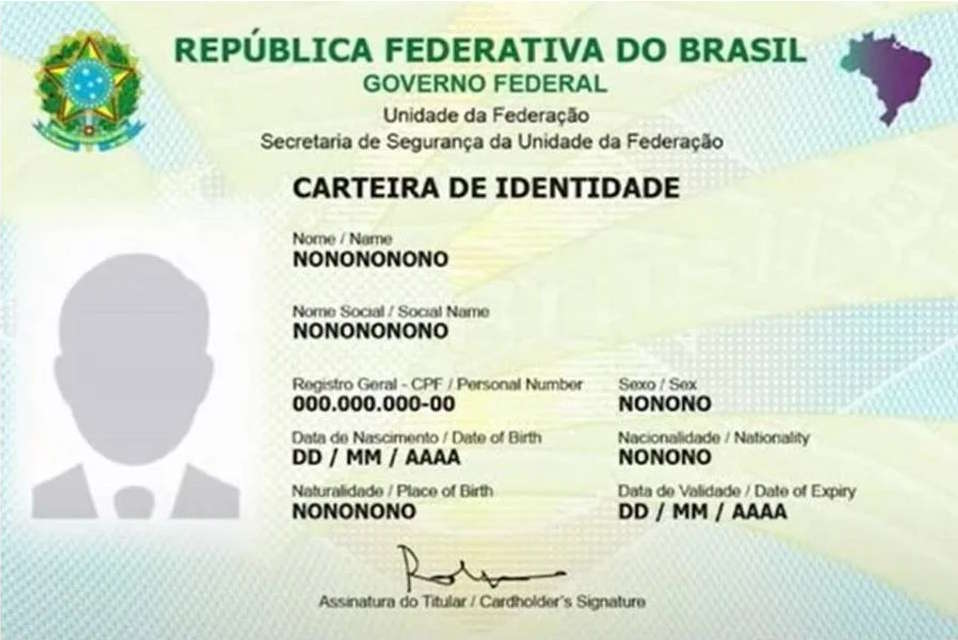
\includegraphics[width=0.18\textwidth]{images-apresentacao/CIN_EXEMPLO.jpg}};
\end{tikzpicture}
\end{center}
\end{frame}

\begin{frame}{Contexto - Importância da Classificação da Imagem}
\begin{columns}
\column{0.5\textwidth}
\begin{itemize}
    \item Assegurar que o documento está correto
    \item Documentos não-digitais
    \item Evita fraudes
\end{itemize}

\column{0.5\textwidth}
\pause
\begin{center}
    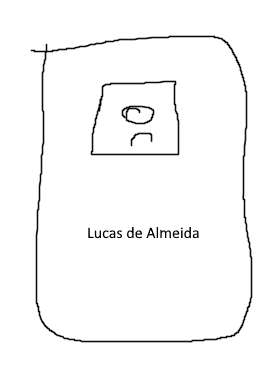
\includegraphics[width=.6\textwidth]{images-apresentacao/EXEMPLO_FRAUDE_CIN.jpg}
\end{center}
\end{columns}
\end{frame}


\begin{frame}{Contexto - Importância da Classificação}
\begin{columns}
\column{0.5\textwidth}
\textbf{Classificação Tradicional:}
\begin{itemize}
    \item Categorização em classes predefinidas
    \item Cross-Entropy Loss
\end{itemize}

\textbf{Desempenho Atual:}
\begin{itemize}
    \item Bakkali et al. (2021): 97.70\% de acurácia no RVL-CDIP
\end{itemize}

\column{0.5\textwidth}
\pause
\textbf{O Problema:}
\begin{itemize}
    \item Novos layouts de documentos
    \item Classes completamente novas
    \item Necessidade de retreinamento
    \item Semanas/meses de engenharia de dados e treinamento
\end{itemize}

% \textbf{Solução:}
% \begin{itemize}
%     \item Técnicas de Zero-Shot Learning (ZSL)
%     \item Generalização para classes não vistas
% \end{itemize}
\end{columns}
\end{frame}

\begin{frame}{Solução}
    \begin{center}
        {\Huge \textbf{Zero-Shot Learning}}\\ \vspace{0.5cm}
        Permite que o modelo reconheça elementos de\\ classes nunca vistas no treinamento
    \end{center}
\end{frame}

\begin{frame}{Sobre a Pesquisa}
\begin{block}{Desafios}
    
    \begin{itemize}
        \item {\large Falta de dataset especializado}
        \begin{itemize}
            \item Imagens de Documento
            \item Generalização
            \item Divisão treino e teste zero-shot
        \end{itemize}
        \item {\large Ausência de metodologia estado-da-arte}
        \begin{itemize}
            \item Paradigma ZSL
            \item Capacidade de classificar
        \end{itemize}
    \end{itemize}
    
\end{block}
\end{frame}

\begin{frame}{Sobre a Pesquisa}
\begin{block}{Contribuições}
    \begin{enumerate}
        \item \textbf{Novo dataset LA-CDIP}
        \begin{itemize}
            \item Classificação ZSL
            \item Derivado do RVL-CDIP
        \end{itemize}
        
        \item \textbf{Abordagem de Visual Document Matching (VDM)}
        \begin{itemize}
            \item Similaridade de documentos
            \item Metric Learning
            \item Generalização Zero-Shot
        \end{itemize}
        
        \item \textbf{Avaliação sistemática}
        \begin{itemize}
            \item Benchmark extensivo
            \item Comparação com LLM
        \end{itemize}
    \end{enumerate}
\end{block}
\end{frame}

% ============================================
% SECTION 2: Methodology
% ============================================
\section{Metodologia}

\begin{frame}{LA-CDIP Dataset - Construção}
\begin{columns}
\column{0.5\textwidth}
\textbf{Motivação:}
\begin{itemize}
    \item RVL-CDIP inadequado para ZSL
    \item Classes definidas por propósito
    \item Múltiplos subclasses por classe
\end{itemize}

\textbf{Solução - LA-CDIP:}
\begin{itemize}
    \item Foco em padrões estruturais
    \item Reorganização do RVL-CDIP
    \item Classes baseadas em layout visual
\end{itemize}

\column{0.5\textwidth}
\includegraphics[width=\textwidth]{images/class_comparison1.png}
\vspace{0.2cm}
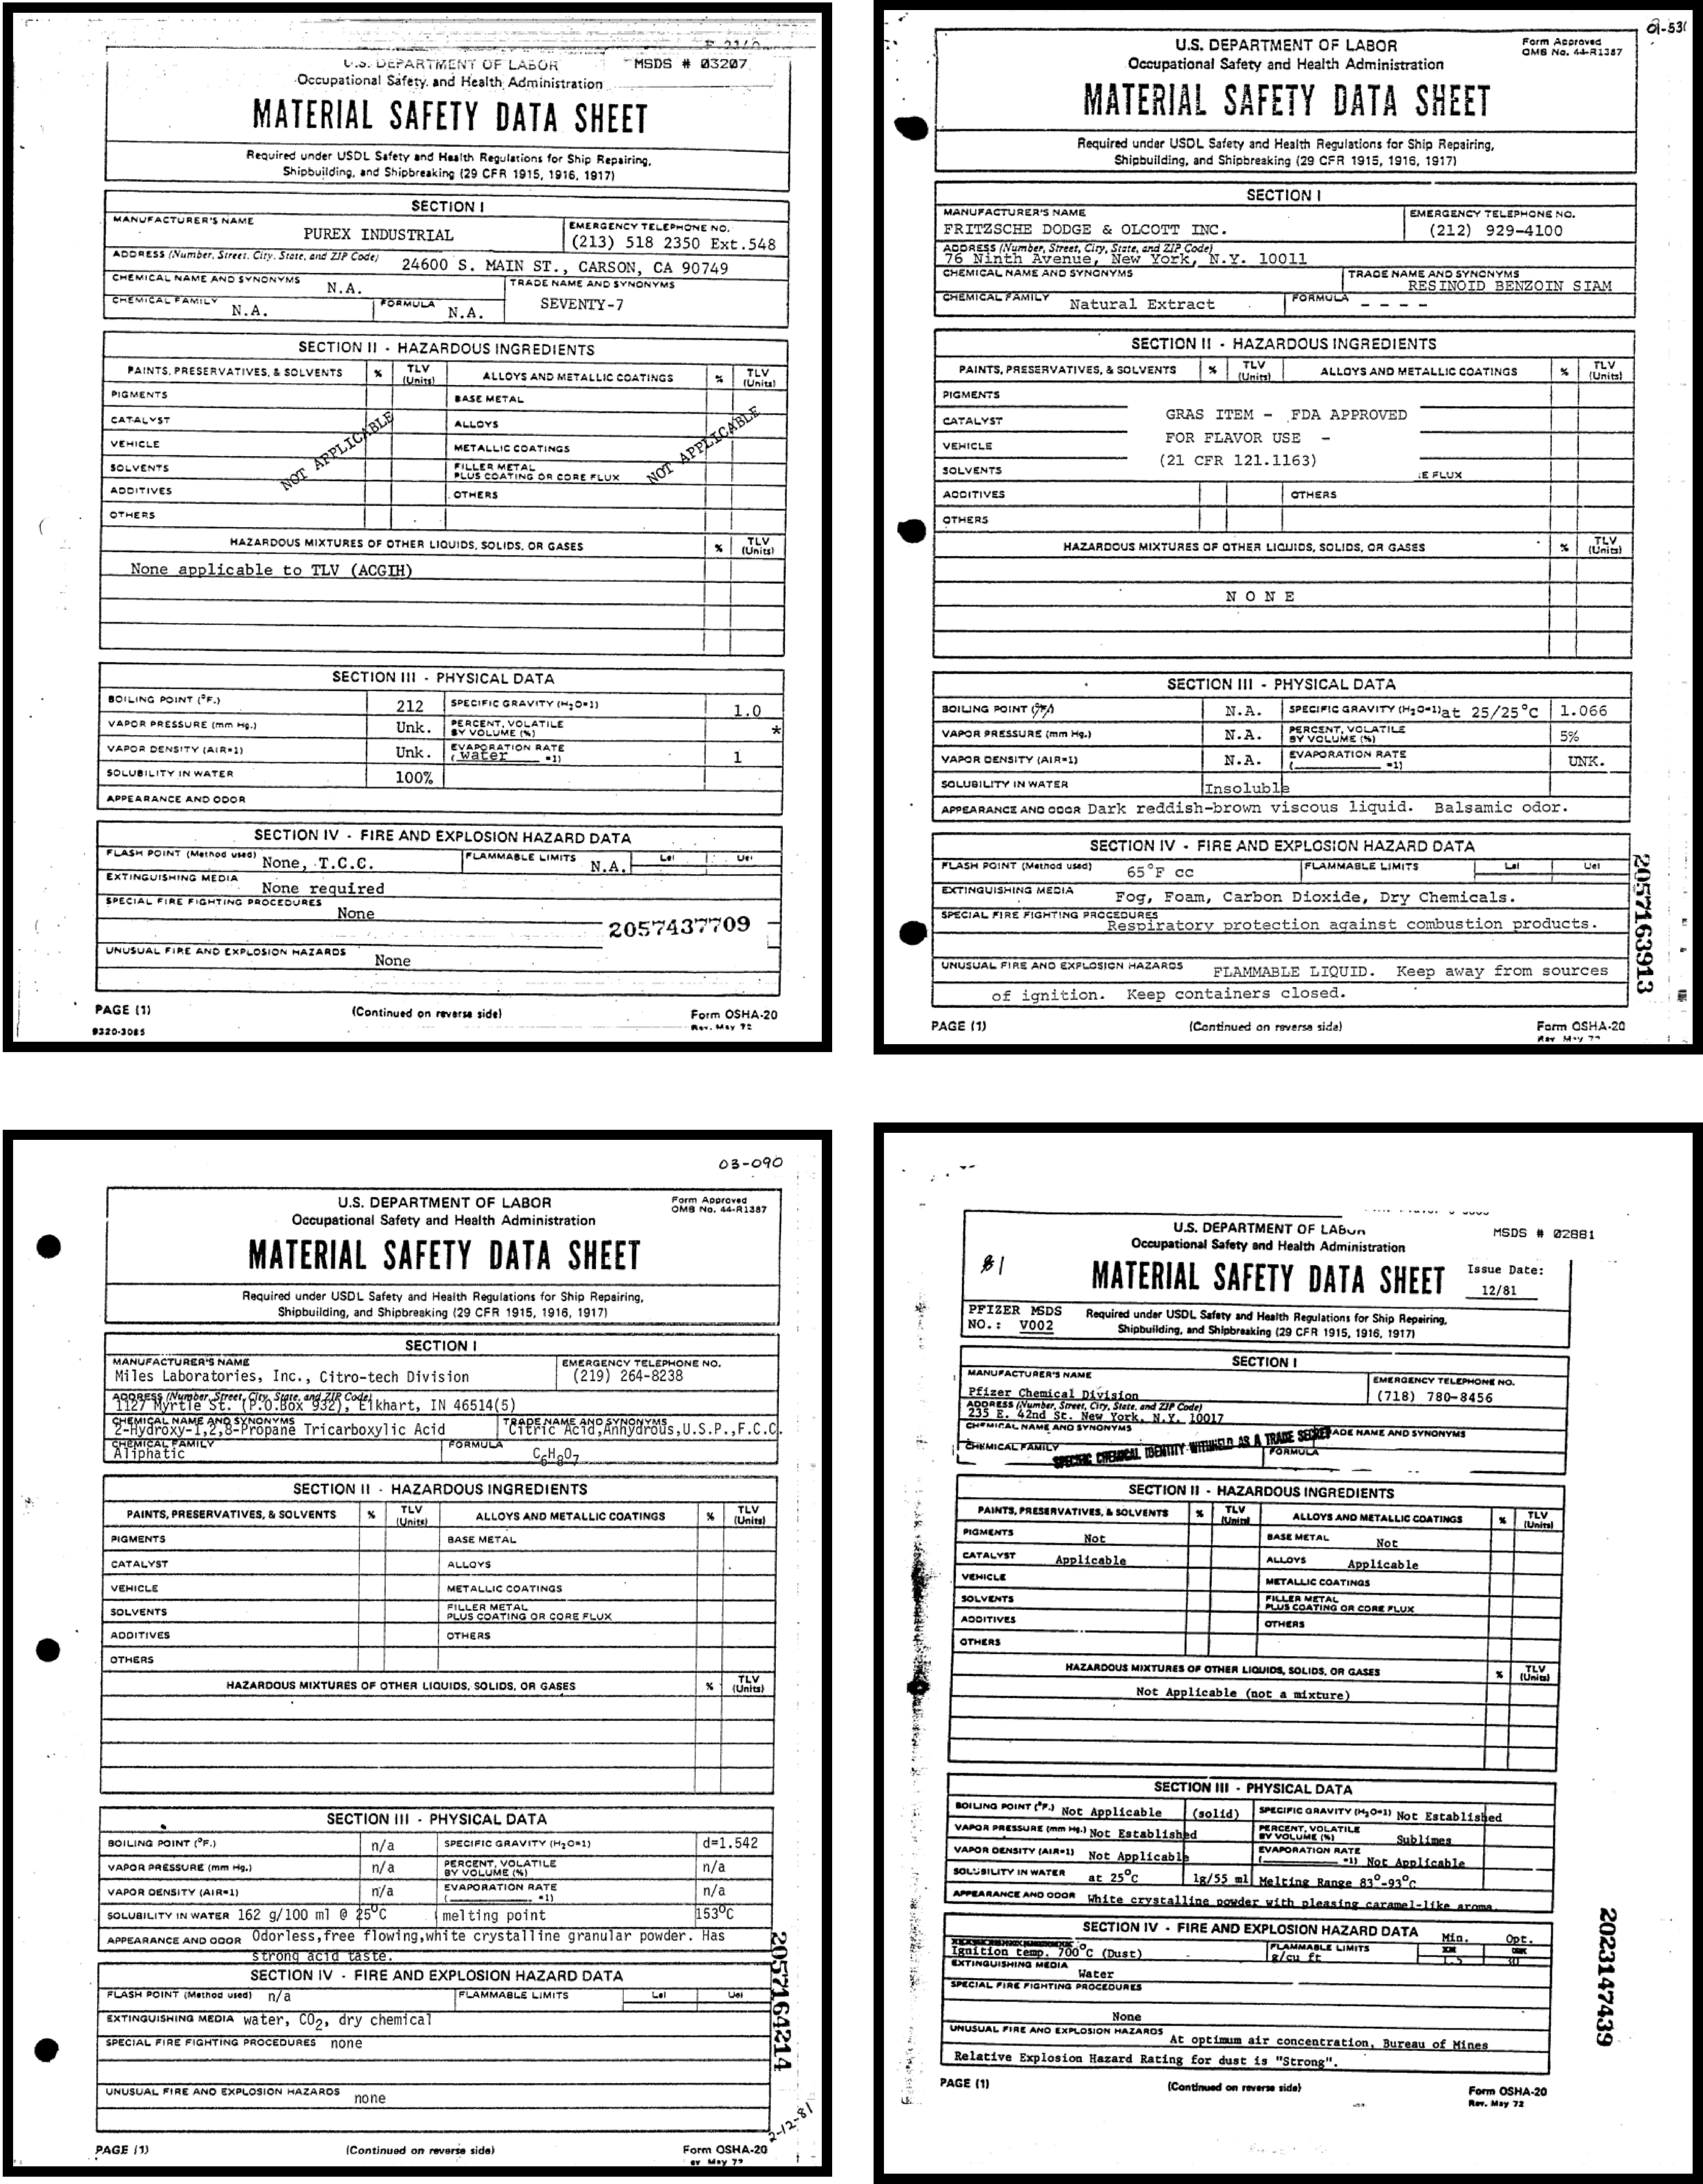
\includegraphics[width=\textwidth]{images/class_comparison2.png}
\end{columns}
\end{frame}

\begin{frame}{LA-CDIP Dataset - Processo de Labeling}
\begin{block}{Framework de Active Learning}
\textbf{Etapa 1: Clustering Preliminar}
\begin{itemize}
    \item Modelo privado de metric learning
    \item Hierarchical Agglomerative Clustering com estratégia de Ward
    \item Número dinâmico de clusters
\end{itemize}

\textbf{Etapa 2: Reorganização Manual}
\begin{itemize}
    \item Limpeza dos clusters (um padrão por cluster)
    \item Merge de clusters com padrões similares
    \item Validação independente para consistência intra e inter-classe
\end{itemize}
\end{block}
\end{frame}

\begin{frame}{Visual Document Matching - Arquitetura}
\begin{columns}
\column{0.6\textwidth}
\textbf{Abordagem:}
\begin{itemize}
    \item Siamese Networks
    \item Metric Learning
    \item Mapeamento para espaço de features
\end{itemize}

\textbf{Backbones Testados:}
\begin{itemize}
    \item ResNet (18, 34, 50, 101, 152)
    \item EfficientNet (B0-B3)
    \item MobileNetV3 (Small, Large)
    \item VGG (11, 13, 16, 19)
    \item Vision Transformer (Base, Large)
\end{itemize}

\column{0.4\textwidth}
\textbf{Princípio:}
\begin{center}
Documentos similares\\
$\downarrow$\\
Pequena distância\\
no espaço de features\\
\vspace{0.3cm}
Documentos diferentes\\
$\downarrow$\\
Grande distância\\
no espaço de features
\end{center}
\end{columns}
\end{frame}

\begin{frame}{Visual Document Matching - Ilustração}
\begin{center}
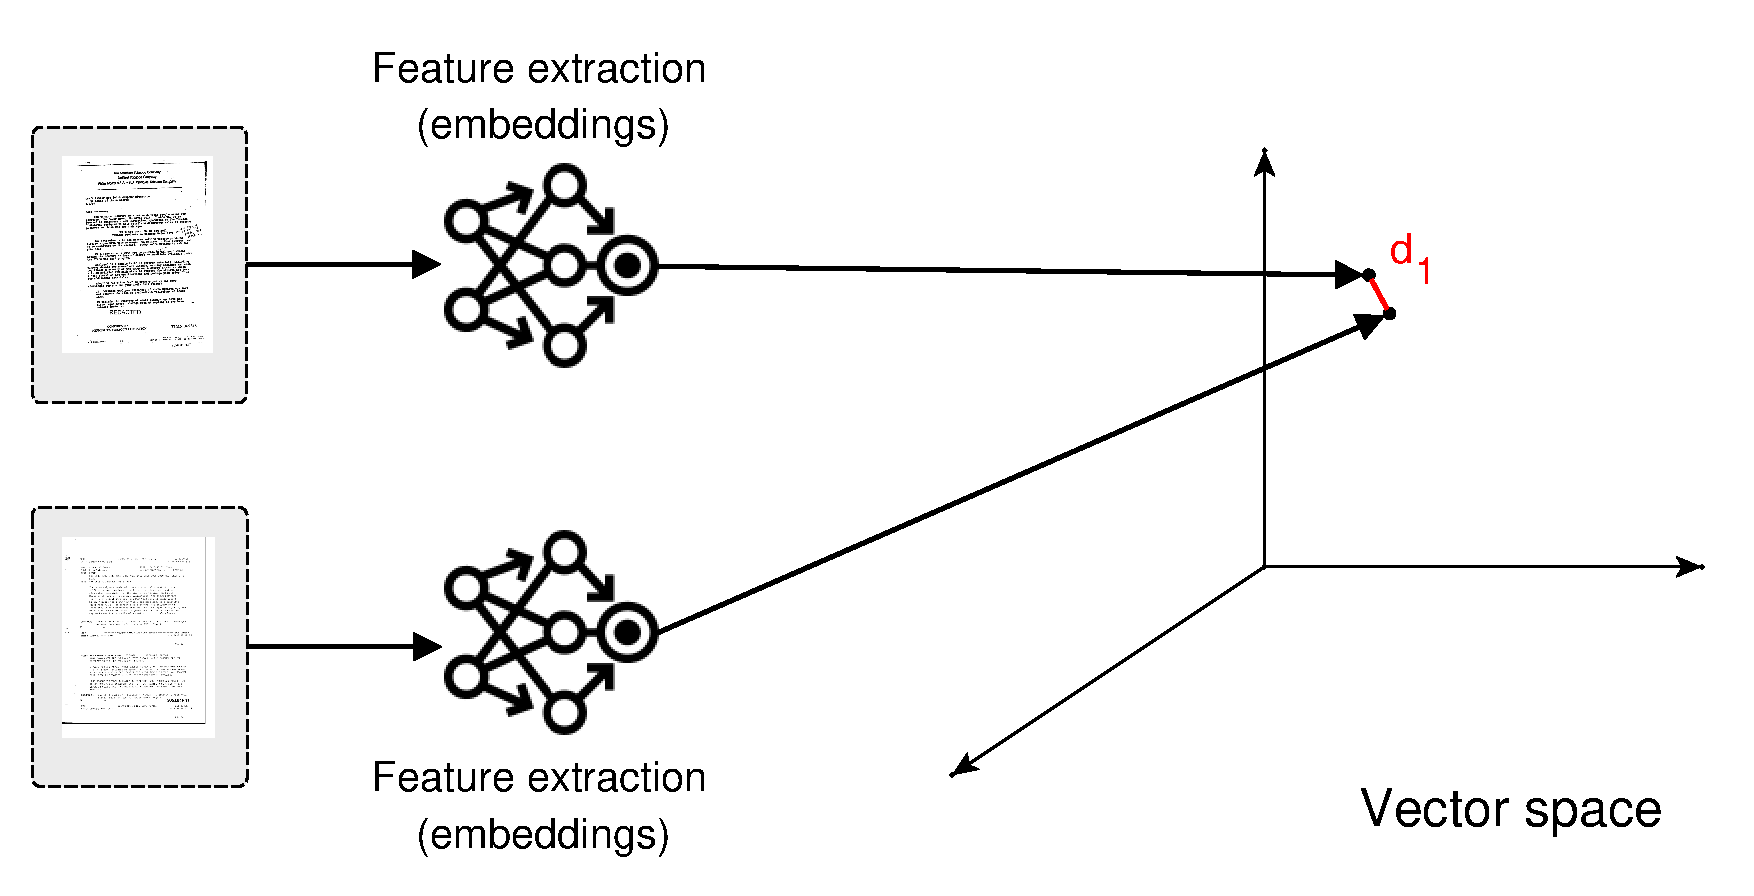
\includegraphics[width=0.8\textwidth]{images/vector_space_1.pdf}
\vspace{0.3cm}
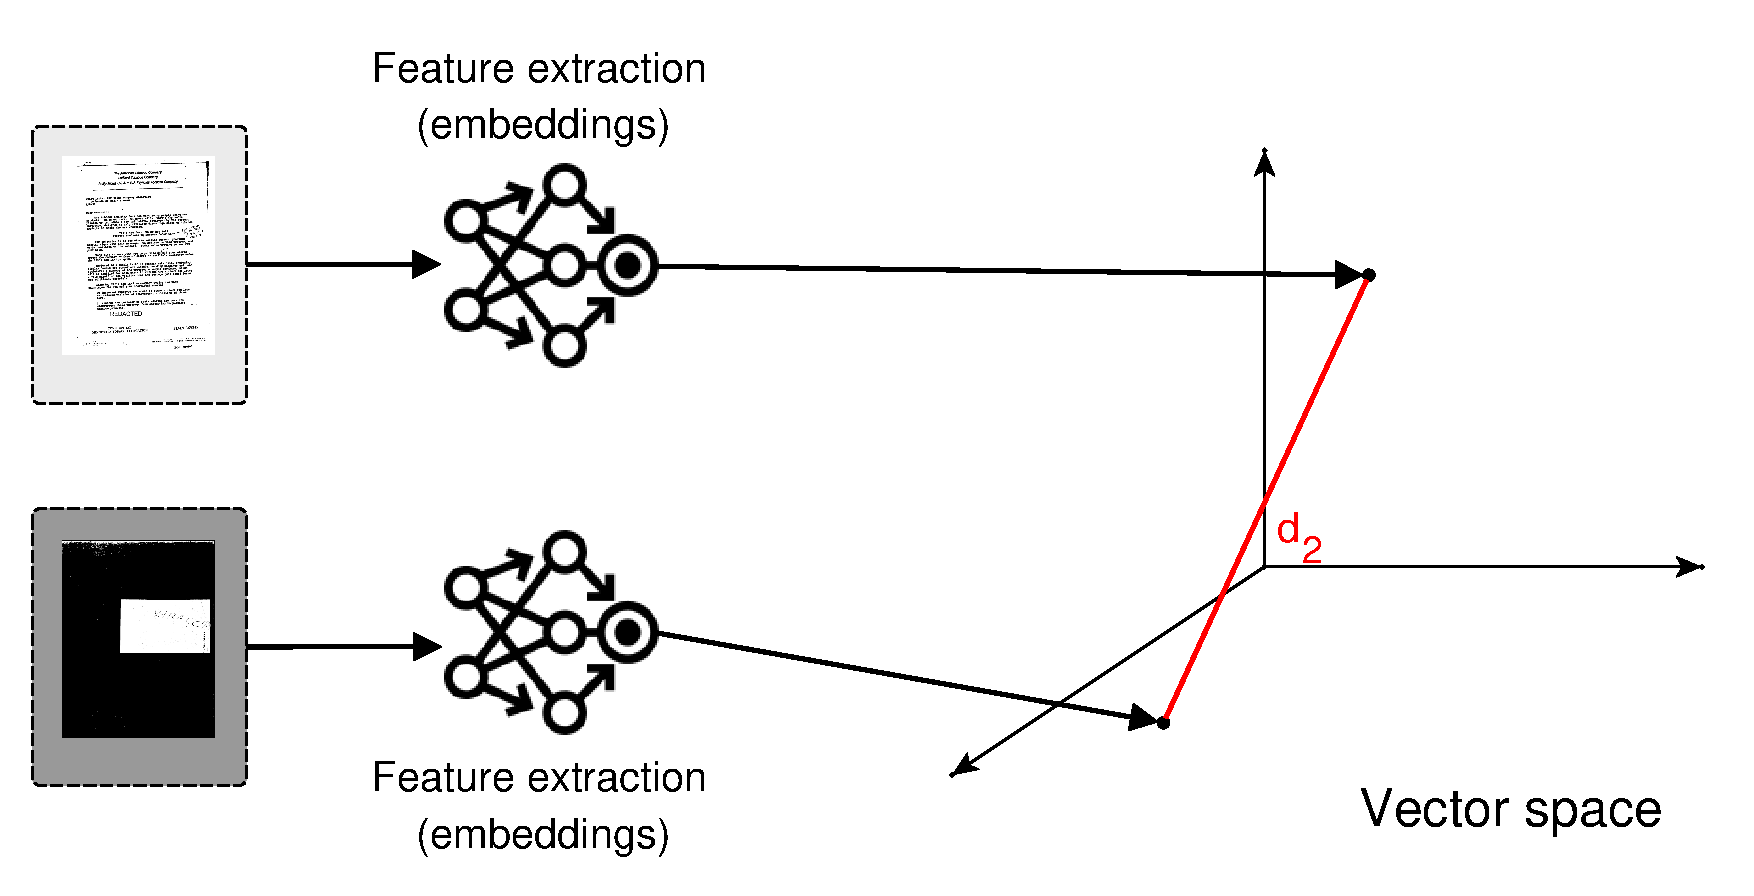
\includegraphics[width=0.8\textwidth]{images/vector_space_2.pdf}
\end{center}
\end{frame}

\begin{frame}{Pipeline de Treinamento}
\begin{block}{Configuração}
\begin{itemize}
    \item \textbf{Input:} Matriz RGB da imagem do documento
    \item \textbf{Pré-processamento:}
    \begin{itemize}
        \item Resize para (224, 224) para maioria dos modelos
        \item Normalização de 0--255 para 0--1
        \item Normalização com média e desvio padrão do split de treino
    \end{itemize}
    \item \textbf{Treinamento:}
    \begin{itemize}
        \item Formação de pares aleatórios
        \item Mesma probabilidade para todas as classes
        \item Contrastive Loss
        \item Sem data augmentation ou pair mining
    \end{itemize}
\end{itemize}
\end{block}
\end{frame}

\begin{frame}{Benchmarking com LLMs}
\begin{columns}
\column{0.5\textwidth}
\textbf{Modelos Avaliados:}
\begin{itemize}
    \item LLaVA 3.2 Vision
    \item InternVL 2.5
    \item Qwen2.5-VL
    \item GPT-4o (2024-11-20)
    \item GPT-4o-mini (2024-07-18)
\end{itemize}

\textbf{Avaliação:}
\begin{itemize}
    \item Zero-shot (sem fine-tuning)
    \item Pontuação de similaridade 0--100
    \item 5 níveis de categorização
\end{itemize}

\column{0.5\textwidth}
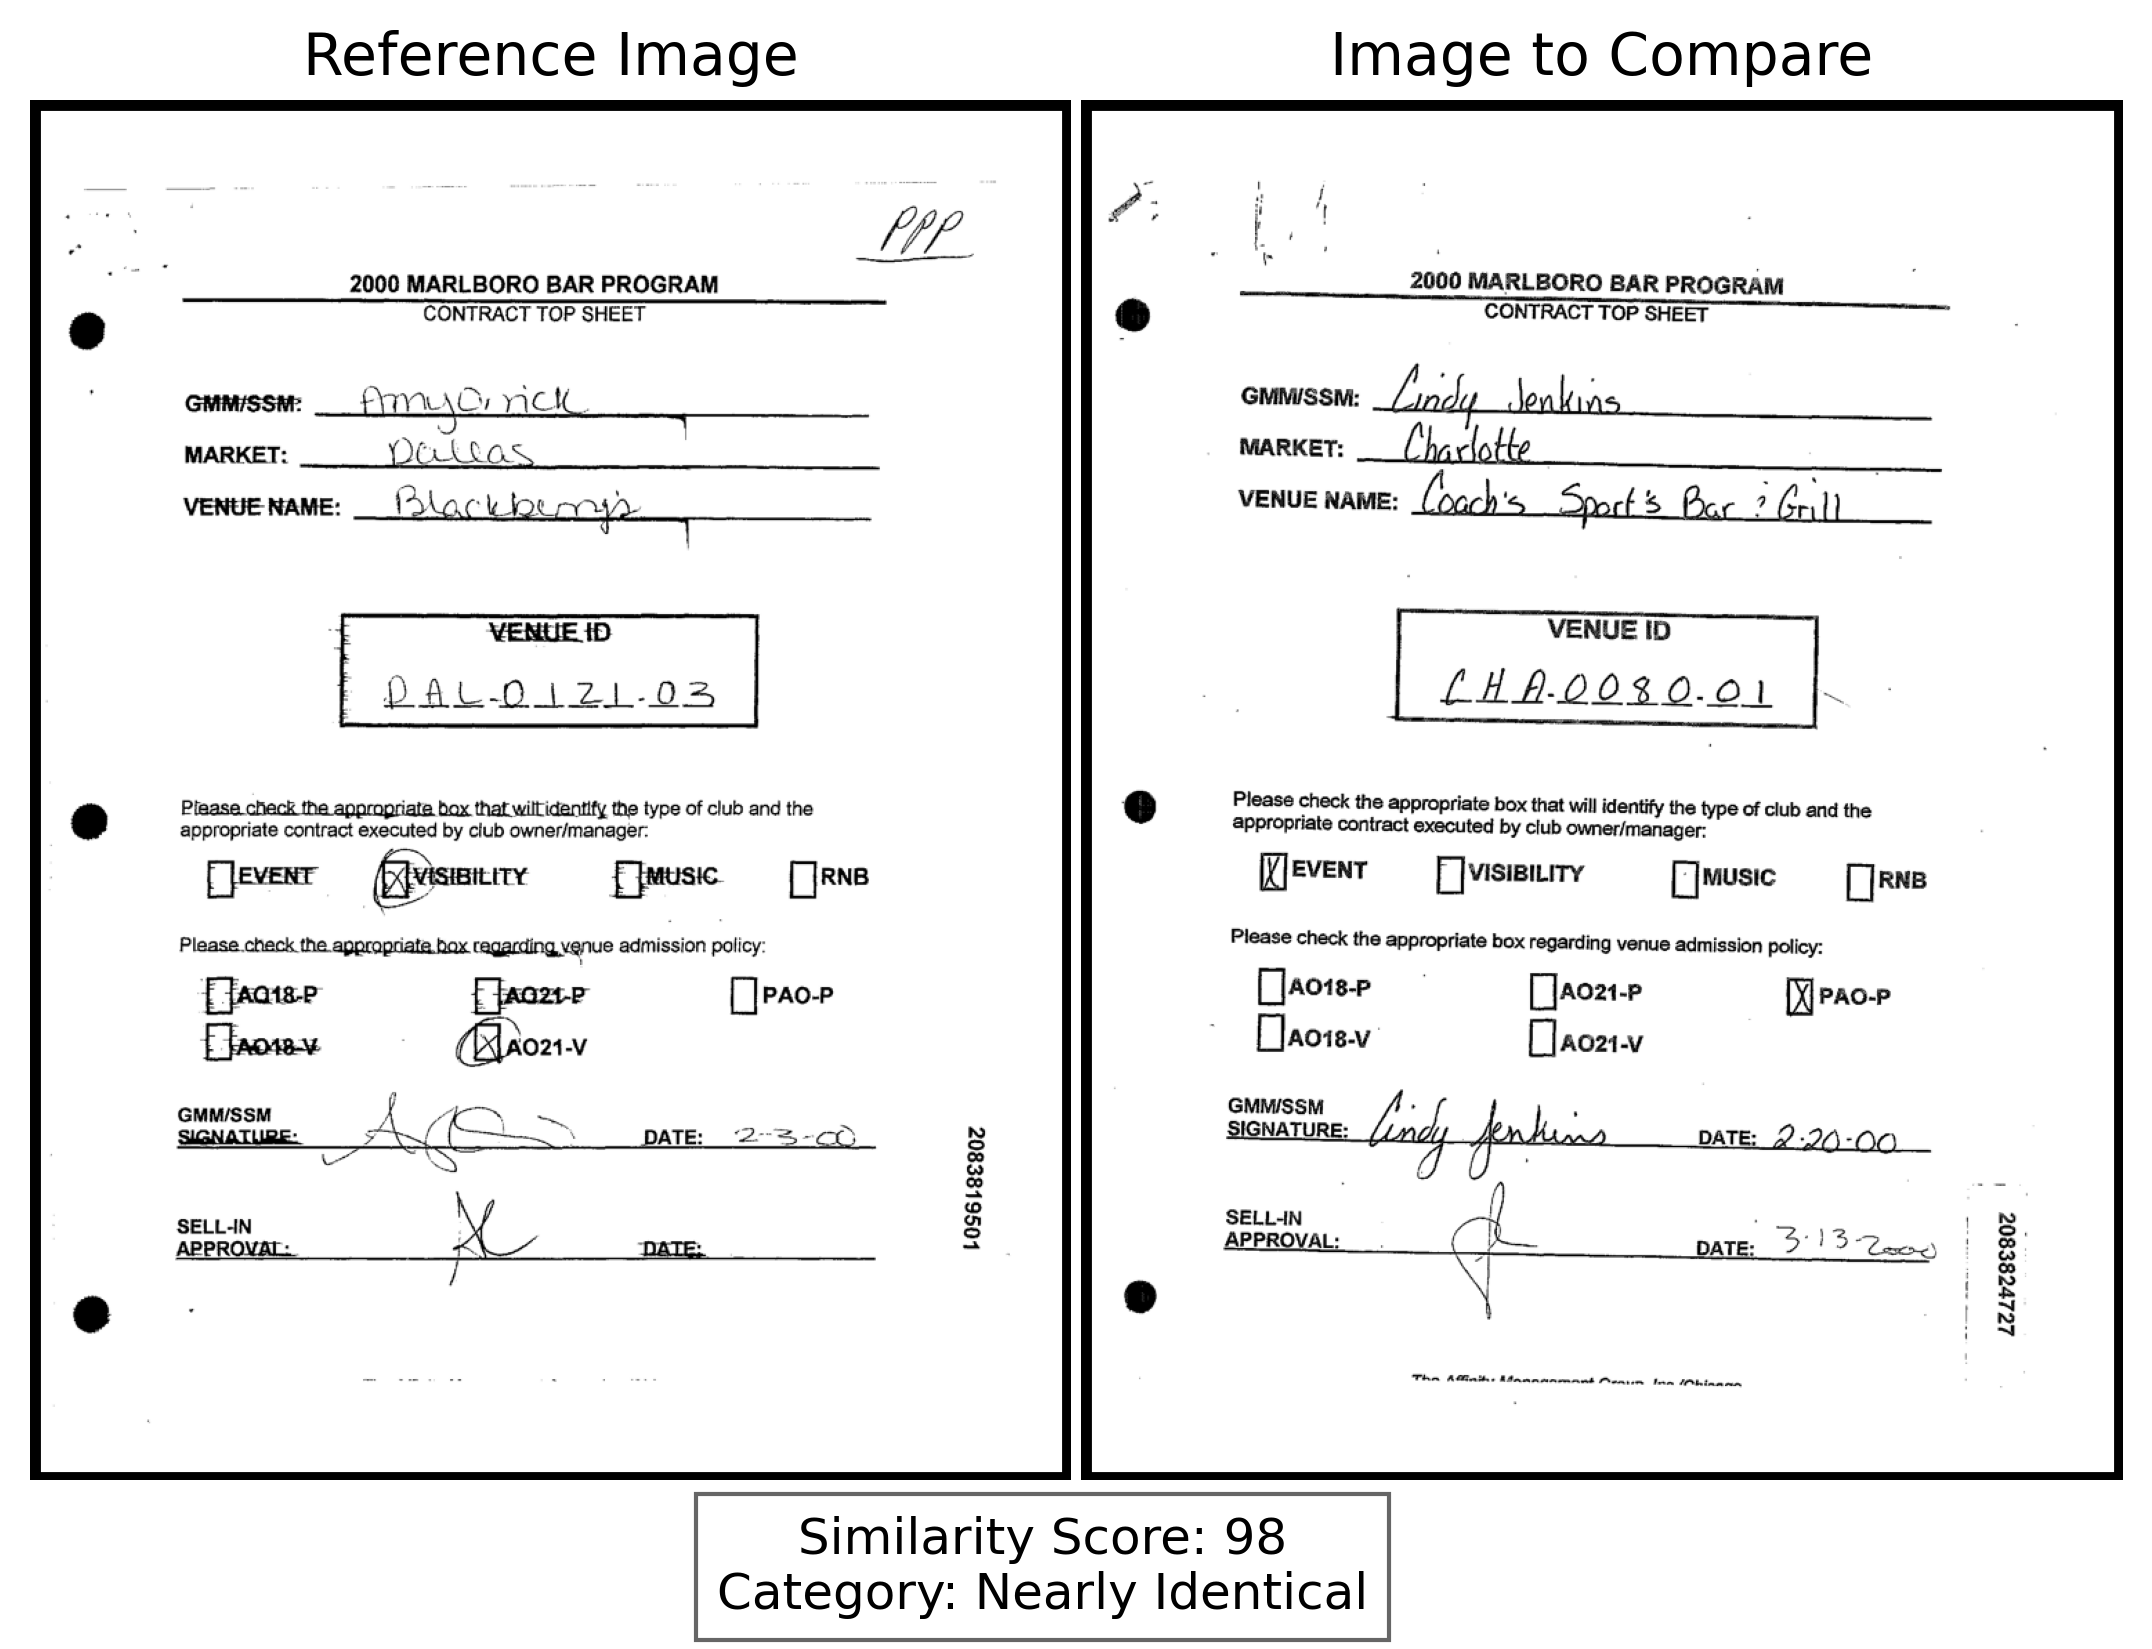
\includegraphics[width=\textwidth]{images/similar.png}
\vspace{0.2cm}
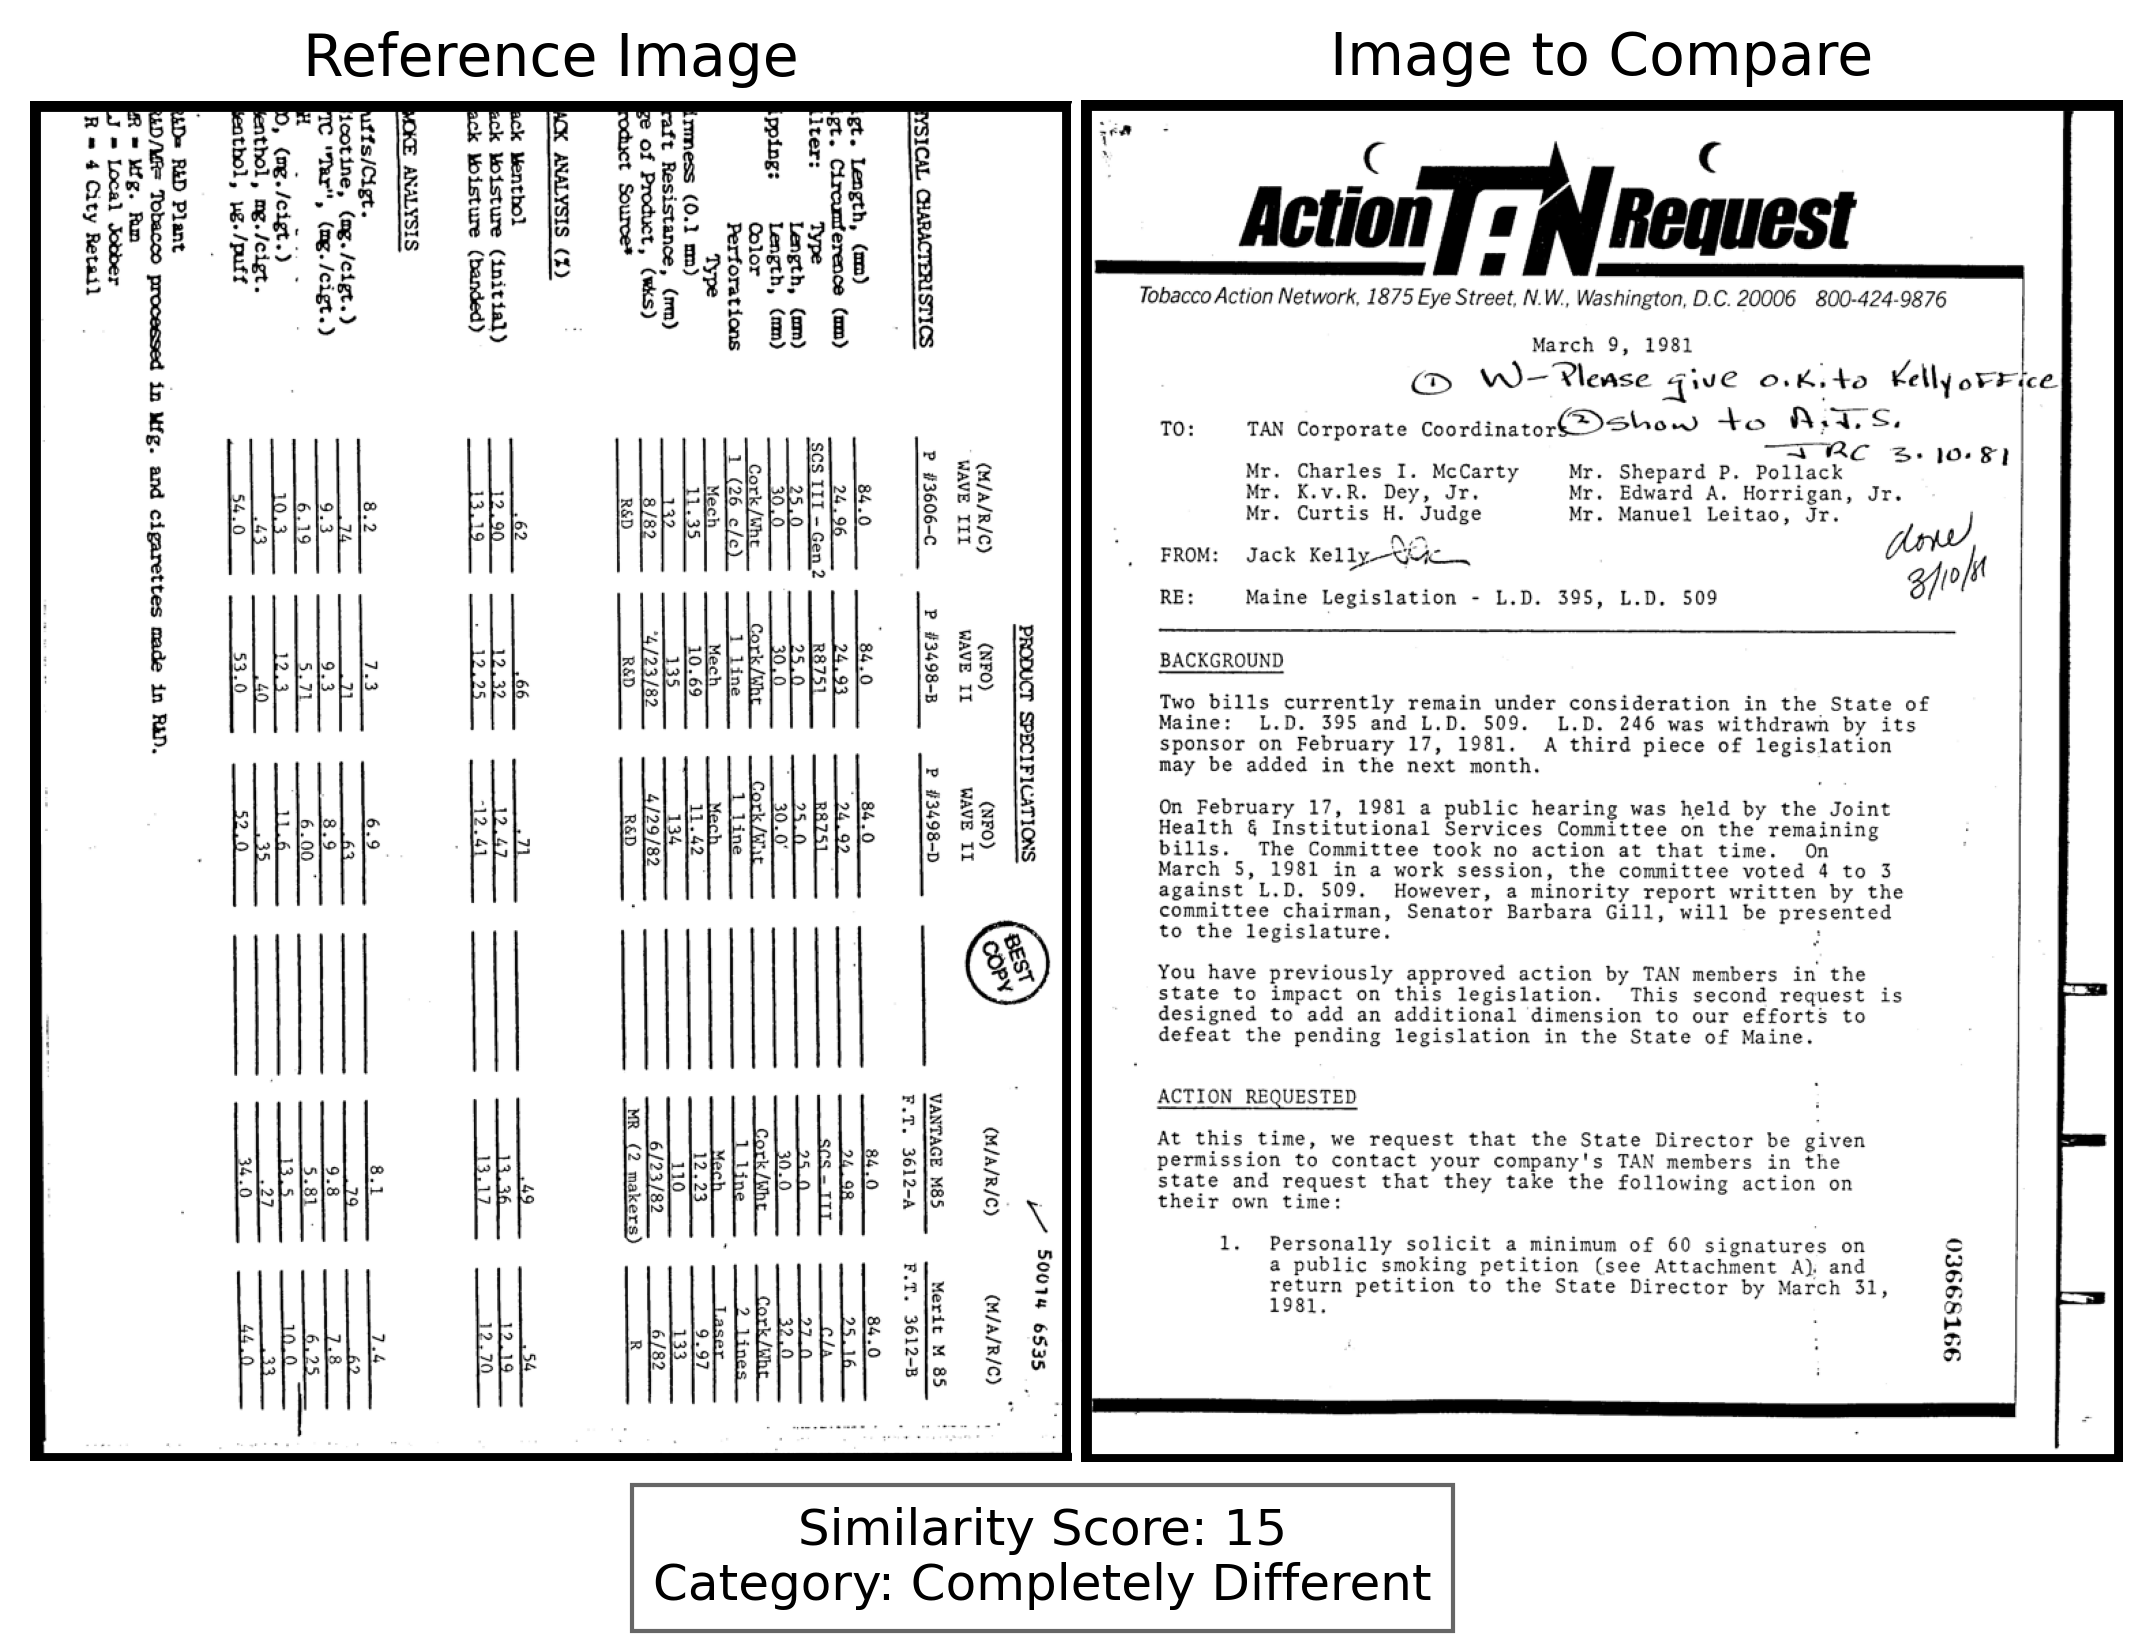
\includegraphics[width=\textwidth]{images/different.png}
\end{columns}
\end{frame}

% ============================================
% SECTION 3: Results
% ============================================
\section{Resultados}

\begin{frame}{LA-CDIP Dataset - Estatísticas}
\begin{columns}
\column{0.5\textwidth}
\textbf{Composição:}
\begin{itemize}
    \item 4.993 documentos
    \item 144 classes diferentes
    \item Min: 2 documentos/classe
    \item Max: 497 documentos/classe
    \item Mediana: 13 documentos/classe
\end{itemize}

\textbf{Splits:}
\begin{itemize}
    \item ZSL: separação completa treino/teste
    \item GZSL: 50\% overlap de classes
    \item 5-fold cross-validation
\end{itemize}

\column{0.5\textwidth}
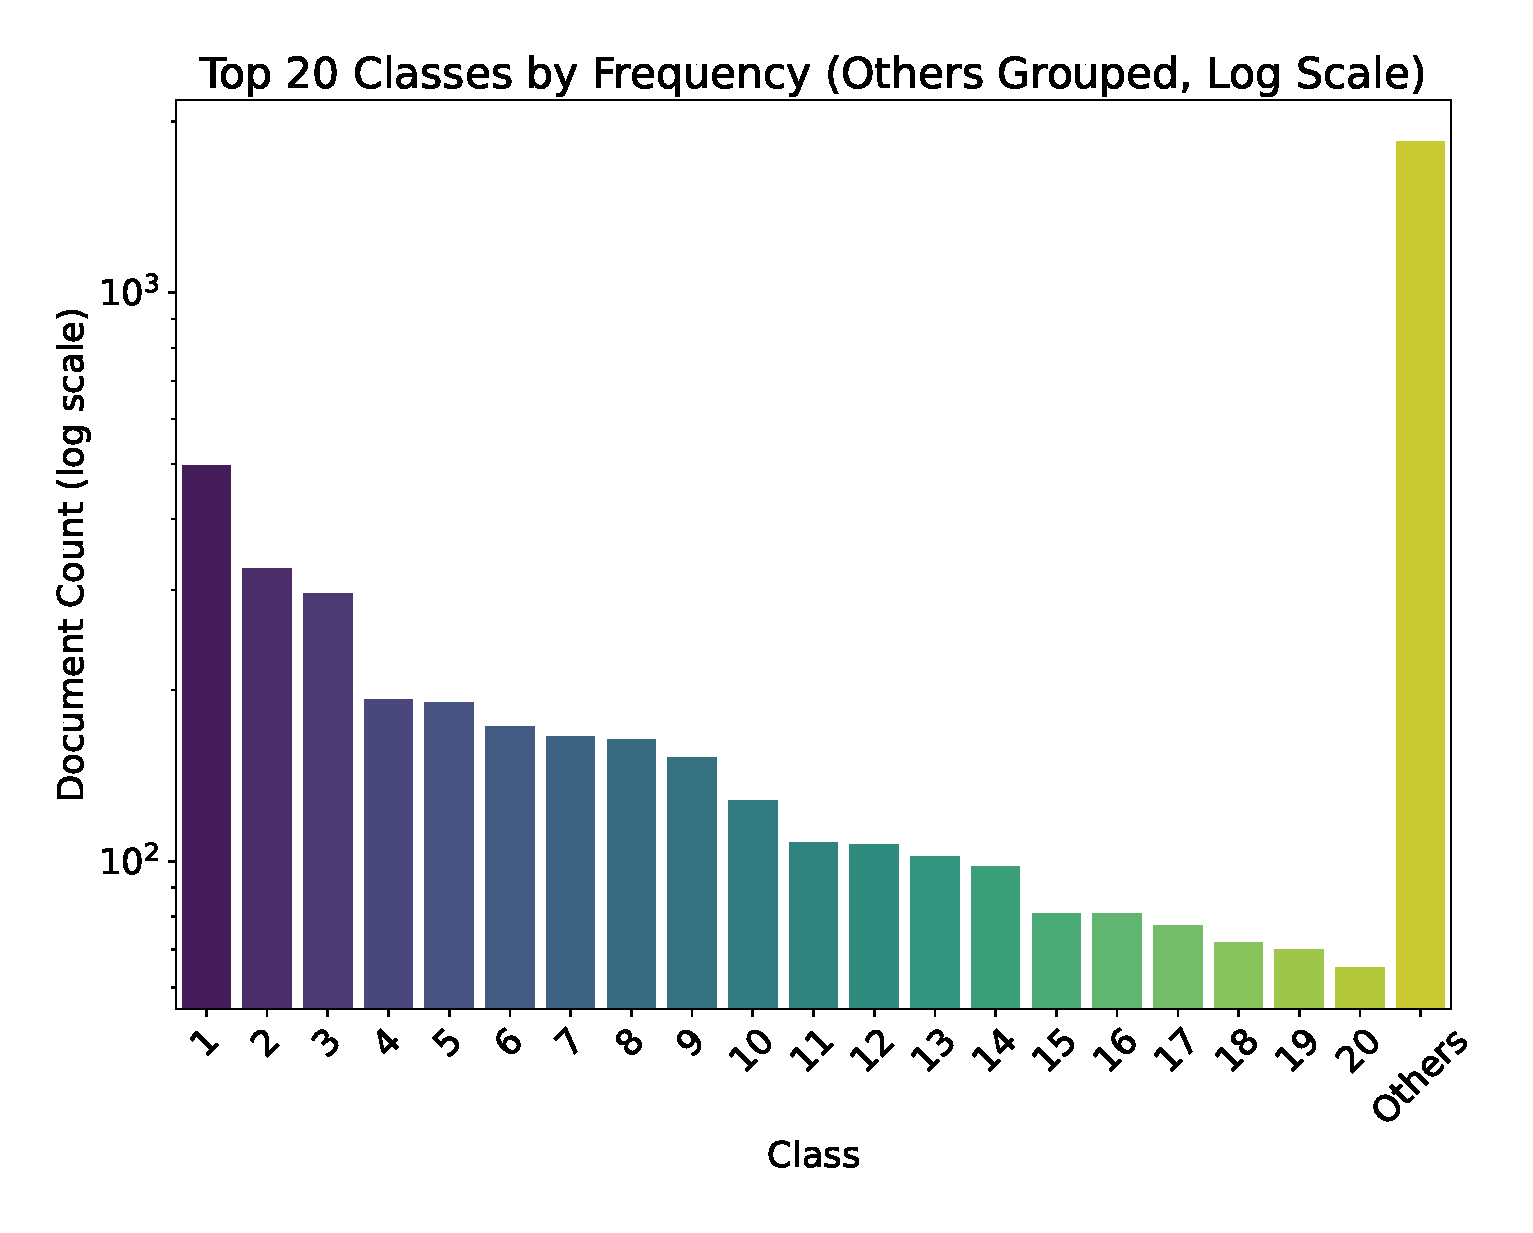
\includegraphics[width=\textwidth]{images/hist2.eps}
\end{columns}
\end{frame}

\begin{frame}{Métricas de Avaliação}
\begin{block}{Equal Error Rate (EER)}
\begin{itemize}
    \item Ponto onde FAR = FRR
    \item FAR: False Acceptance Rate
    \item FRR: False Rejection Rate
\end{itemize}
\end{block}

\begin{columns}
\column{0.5\textwidth}
\begin{equation*}
FAR(\tau) = \frac{\text{False Acceptances}}{\text{Total Negatives}}
\end{equation*}

\column{0.5\textwidth}
\begin{equation*}
FRR(\tau) = \frac{\text{False Rejections}}{\text{Total Positives}}
\end{equation*}
\end{columns}

\vspace{0.3cm}
\begin{center}
\textbf{Protocolo de Teste:}\\
Para cada documento: 1 par similar + 1 par dissimilar
\end{center}
\end{frame}

\begin{frame}{Resultados - Visão Geral}
\begin{table}
\tiny
\begin{tabular}{lclcccc}
\toprule
\textbf{Architecture} & \textbf{Edition} & \textbf{Params} & \textbf{ZSL CV} & \textbf{GZSL CV} & \textbf{Test ZSL} & \textbf{Test GZSL} \\
\midrule
ResNet & 18 & 11M & 5.03 & 1.54 & 4.98 & 1.51 \\
ResNet & 34 & 21M & 4.32 & 2.10 & 4.13 & 1.53 \\
EfficientNet & 0 & 4M & 4.41 & 2.27 & 6.02 & 0.95 \\
EfficientNet & 1 & 6M & 3.93 & 3.54 & 8.88 & 2.70 \\
VGG & 13 & 129M & 7.03 & 4.79 & 9.30 & 3.95 \\
ViT & Base & 87M & 12.43 & 7.97 & 19.72 & 5.19 \\
\midrule
GPT-4o & 2024-11-20 & * & -- & -- & 2.75 & 1.33 \\
GPT-4o mini & 2024-07-18 & * & -- & -- & 4.70 & 4.07 \\
Qwen-VL & 2.5 & 7B & -- & -- & 6.61 & 4.20 \\
InternVL & 2.5 & 8B & -- & -- & 8.58 & 10.40 \\
LLaMA & 3.2 & 11B & -- & -- & 13.95 & 21.90 \\
\bottomrule
\end{tabular}
\caption*{Mean EER (\%) - Valores menores são melhores}
\end{table}
\end{frame}

\begin{frame}{Resultados - Modelos Visuais}
\begin{block}{Principais Observações}
\begin{itemize}
    \item \textbf{Arquiteturas menores superaram as maiores}
    \begin{itemize}
        \item ResNet-18 e ResNet-34: melhor desempenho
        \item ResNet-50, 101, 152: desempenho progressivamente pior
    \end{itemize}
    
    \item \textbf{Vision Transformer (ViT): pior desempenho}
    \begin{itemize}
        \item Overfitting nos dados de treino
        \item 0\% de erro de treino, alto erro de validação
        \item Causa provável: dataset pequeno (4.993 documentos)
    \end{itemize}
    
    \item \textbf{Melhores modelos:}
    \begin{itemize}
        \item ResNet-34, EfficientNet-0 e EfficientNet-1
        \item Balanço entre tamanho e generalização
    \end{itemize}
\end{itemize}
\end{block}
\end{frame}

\begin{frame}{Resultados - Comparação ZSL vs GZSL}
\begin{columns}
\column{0.5\textwidth}
\textbf{GZSL consistentemente melhor:}
\begin{itemize}
    \item 50\% das classes vistas no treino
    \item Maior diferença em modelos grandes
    \item Overfitting mitigado no cenário mais fácil
\end{itemize}

\textbf{Test split ZSL mais desafiador:}
\begin{itemize}
    \item Alta variância entre splits
    \item Padrões completamente diferentes
    \item Taxas de erro mais altas
\end{itemize}

\column{0.5\textwidth}
\textbf{Exemplo ResNet-18:}
\begin{itemize}
    \item ZSL CV: 5.03\%
    \item GZSL CV: 1.54\%
    \item Test ZSL: 4.98\%
    \item Test GZSL: 1.51\%
\end{itemize}

\vspace{0.5cm}
\textbf{Exemplo ViT-Base:}
\begin{itemize}
    \item ZSL CV: 12.43\%
    \item GZSL CV: 7.97\%
    \item Test ZSL: 19.72\%
    \item Test GZSL: 5.19\%
\end{itemize}
\end{columns}
\end{frame}

\begin{frame}{Resultados - Large Language Models}
\begin{block}{Observações}
\begin{itemize}
    \item \textbf{GPT-4o: melhor desempenho geral}
    \begin{itemize}
        \item ZSL: 2.75\% | GZSL: 1.33\%
        \item Porém: centenas de vezes mais caro por inferência
    \end{itemize}
    
    \item \textbf{Alternativas open-source promissoras:}
    \begin{itemize}
        \item Qwen-VL 7B: desempenho próximo ao GPT-4o mini
        \item InternVL 2.5: competitivo
    \end{itemize}
    
    \item \textbf{LLaMA 3.2 Vision:}
    \begin{itemize}
        \item Limitações no manuseio de múltiplas imagens
        \item Necessário combinar imagens em input único
    \end{itemize}
    
    \item \textbf{Tendências diferentes entre cenários:}
    \begin{itemize}
        \item InternVL melhor no ZSL
        \item GPT melhor no GZSL
    \end{itemize}
\end{itemize}
\end{block}
\end{frame}

\begin{frame}{Comparação: Visual Models vs LLMs}
\begin{center}
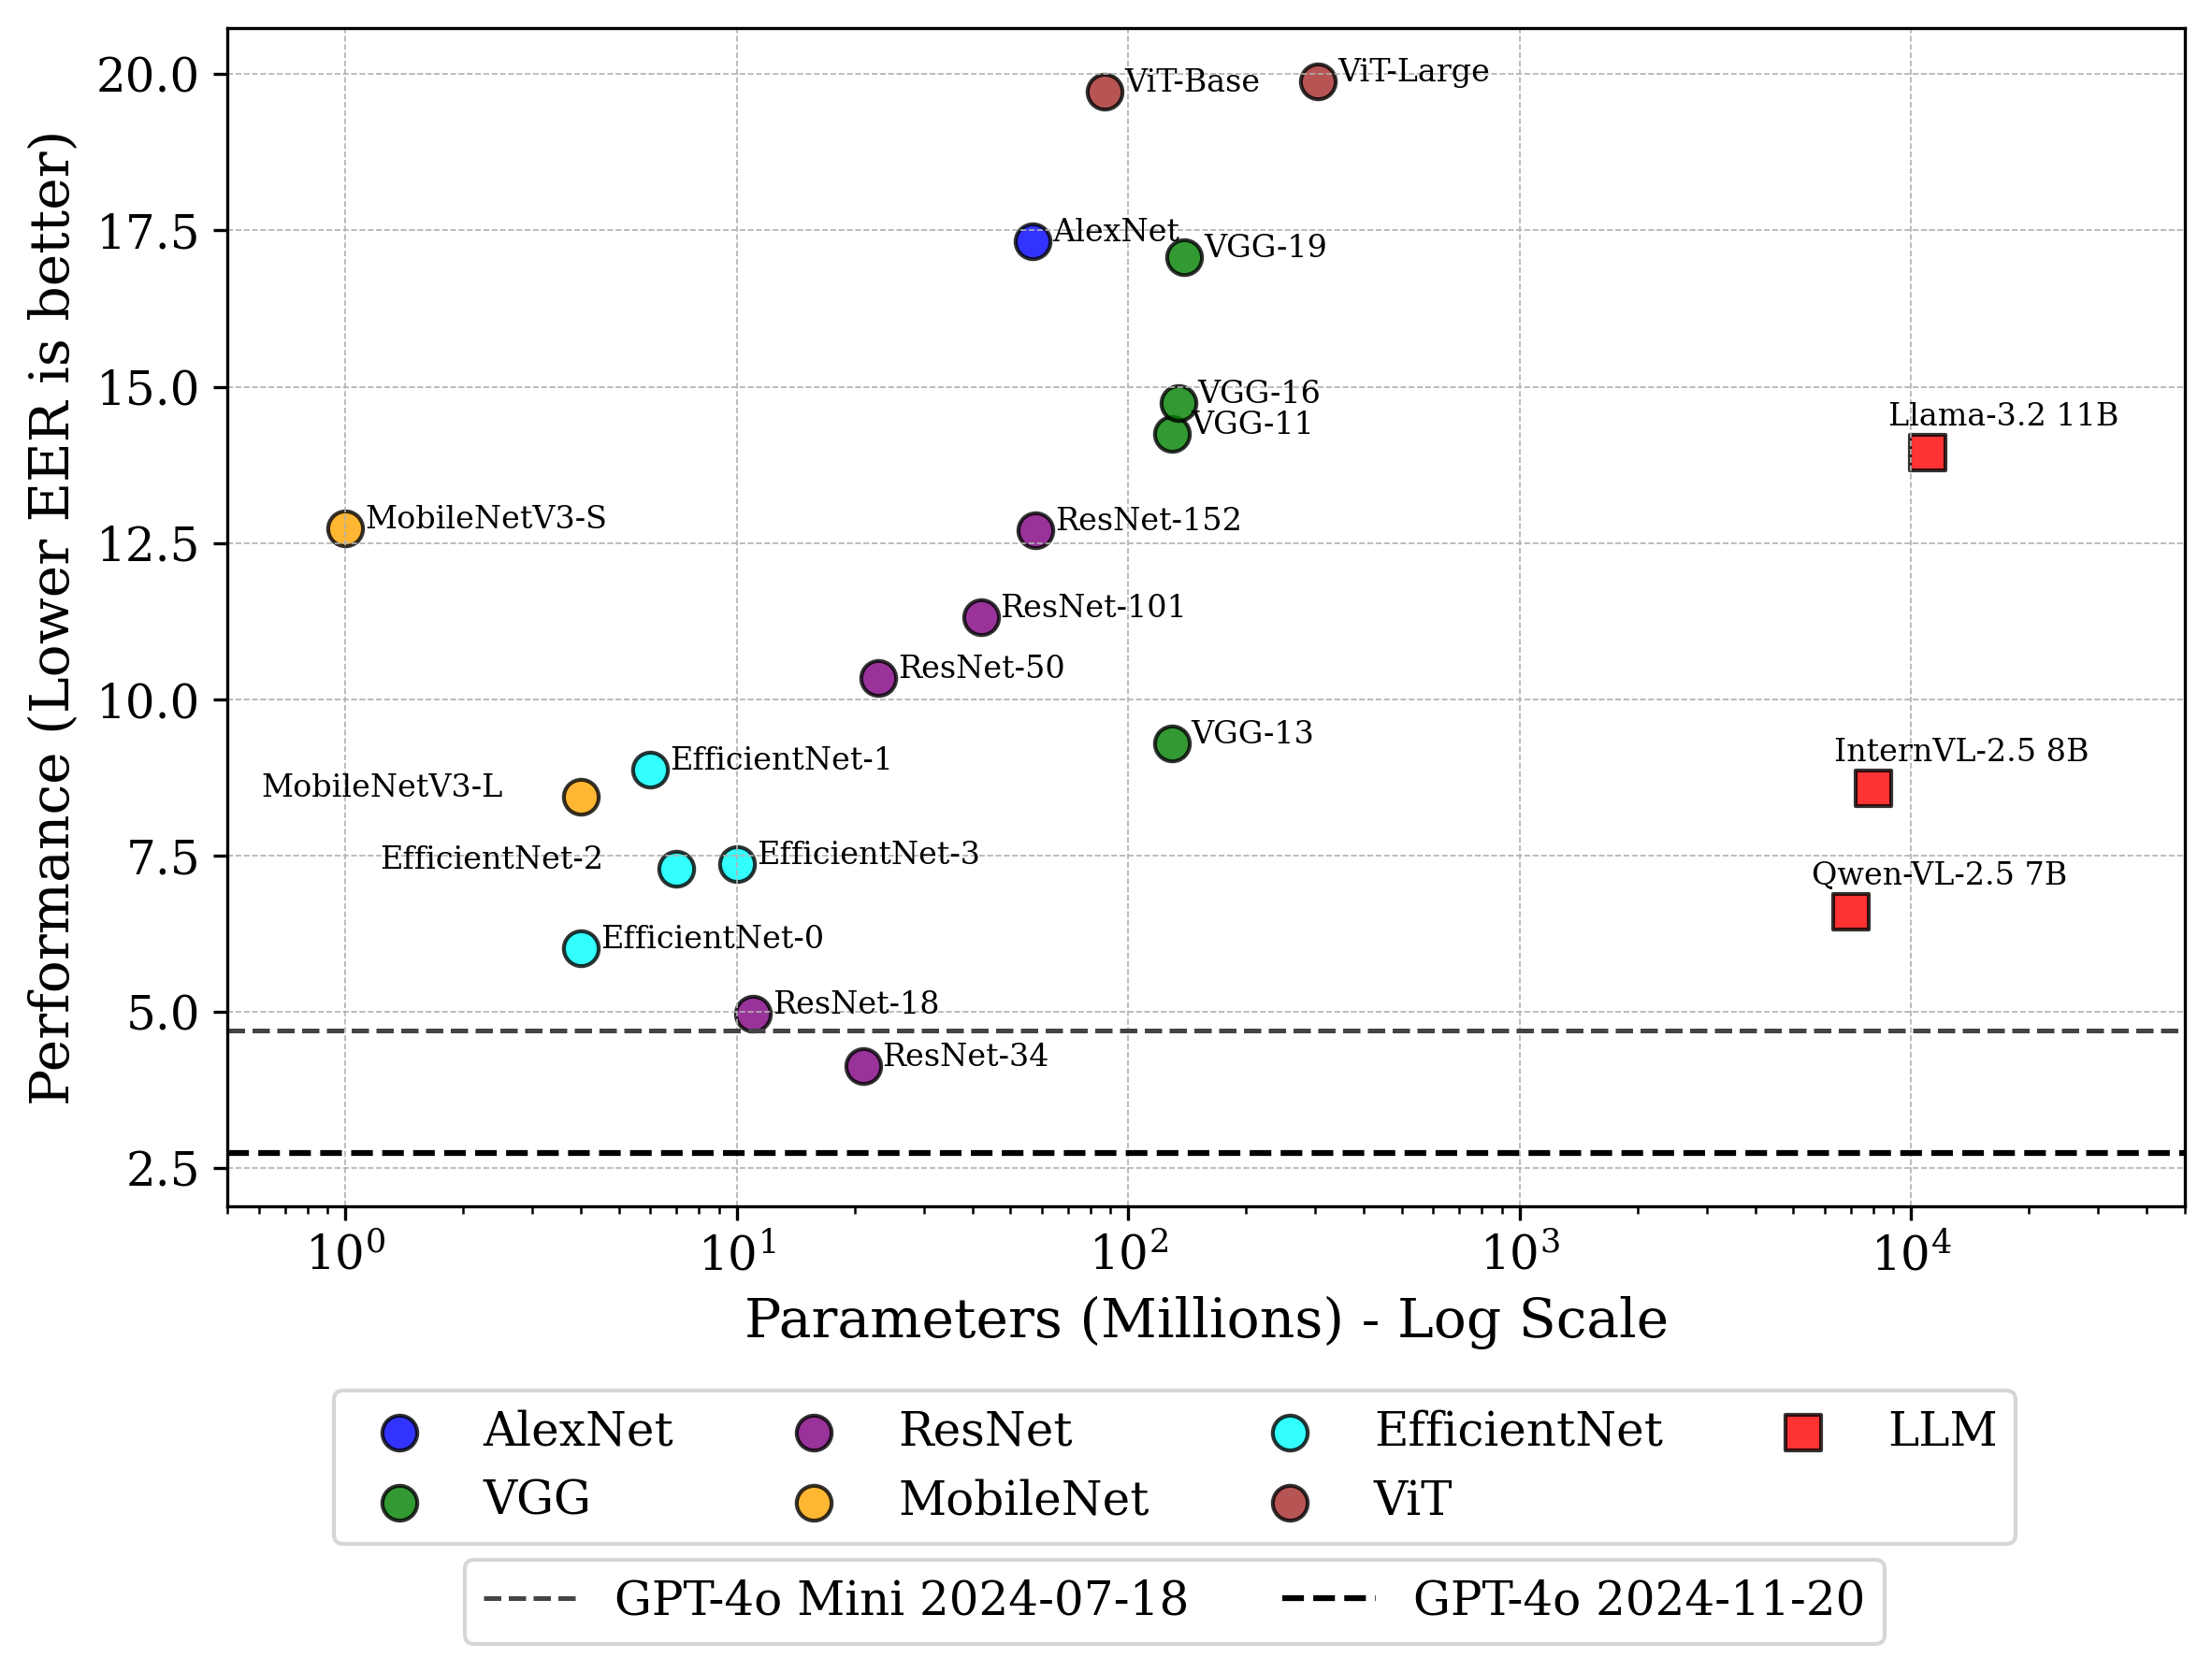
\includegraphics[width=0.85\textwidth]{images/performance_vs_parameters.png}
\end{center}

\textbf{Trade-off entre complexidade e efetividade:}
\begin{itemize}
    \item Modelos visuais leves (ResNet-18, EfficientNet-0): competitivos com muito menos parâmetros
    \item GPT-4o: ligeiro ganho de performance, mas custo muito maior
\end{itemize}
\end{frame}

\begin{frame}{Usos Industriais}
\begin{block}{Sistema de Verificação (Classificação Binária)}
\begin{itemize}
    \item Dado: documento de referência + threshold
    \item Decisão: aceitar se distância < threshold, rejeitar caso contrário
\end{itemize}
\end{block}

\begin{block}{Sistema de Identificação (Classificação Multi-classe)}
\begin{itemize}
    \item Dado: referências para cada classe + threshold
    \item Decisão: atribuir à classe mais próxima ou rejeitar se fora do threshold
\end{itemize}
\end{block}

\textbf{Design Choices:}
\begin{itemize}
    \item Múltiplas referências por classe (usar centroid)
    \item Thresholds diferentes por classe
    \item Armazenar embeddings ao invés de imagens
    \item Complexidade: O(r) verificação, O(rc) identificação
\end{itemize}
\end{frame}

% ============================================
% SECTION 4: Conclusion
% ============================================
\section{Conclusão}

\begin{frame}{Conclusões}
\begin{block}{Principais Contribuições}
\begin{enumerate}
    \item \textbf{LA-CDIP Dataset}
    \begin{itemize}
        \item Dataset categorizado exclusivamente por layout
        \item Alternativa Zero-Shot para classificação de documentos
    \end{itemize}
    
    \item \textbf{Benchmarking Sistemático}
    \begin{itemize}
        \item Diversos backbones visuais estabelecidos
        \item Comparação com LLMs populares
    \end{itemize}
    
    \item \textbf{Resultados Práticos}
    \begin{itemize}
        \item Modelos visuais menores superam LLMs (exceto GPT-4o)
        \item GPT-4o melhor, mas custo-benefício desfavorável
        \item Alternativas open-source viáveis
    \end{itemize}
\end{enumerate}
\end{block}
\end{frame}

\begin{frame}{Limitações e Trabalhos Futuros}
\begin{columns}
\column{0.5\textwidth}
\textbf{Limitações Conhecidas:}
\begin{itemize}
    \item Dataset relativamente pequeno
    \item Complexidade de arquiteturas limitada
    \item Apenas documentos do RVL-CDIP
\end{itemize}

\column{0.5\textwidth}
\textbf{Trabalhos Futuros:}
\begin{itemize}
    \item Aumentar número de amostras
    \item Aumentar número de classes
    \item Incluir fontes adicionais de documentos
    \item Data augmentation
    \item Permitir modelos mais complexos
\end{itemize}
\end{columns}
\end{frame}

\begin{frame}{Timeline da Pesquisa}
\begin{center}
\small
\begin{tabular}{llllll}
\hline
\textbf{Tarefa} & \textbf{5º} & \textbf{6º} & \textbf{7º} & \textbf{8º} & \textbf{9º--10º} \\
\hline
Literatura & \checkmark & & & & \\
Framework & \checkmark & \checkmark & & & \\
Dataset Labeling & & \checkmark & & & \\
Experimentos & & \checkmark & \checkmark & & \\
Produção de Paper & & & & \checkmark & \checkmark \\
Extra Labeling & & & & & \checkmark \\
Qualificação & & & & & \textbf{8º trim} \\
Defesa de Mestrado & & & & & \textbf{10º trim} \\
\hline
\end{tabular}
\end{center}

\vspace{0.5cm}
\begin{center}
\textbf{Status atual: 8º trimestre (Qualificação)}
\end{center}
\end{frame}

% ============================================
% Final Slide
% ============================================
\begin{frame}[plain]
\begin{center}
{\Huge Obrigado!}

\vspace{1cm}

{\Large Perguntas?}

\vspace{1cm}

Lucas de Almeida Bandeira Macedo\\
\texttt{lucasabmacedo@hotmail.com}

\vspace{0.5cm}

Orientador: Prof. Dr. Pedro Garcia Freitas\\
Coorientador: Prof. Dr. Bruno Luiggi Macchiavello Espinoza
\end{center}
\end{frame}


\end{document}
